%% LaTeX Beamer presentation template (requires beamer package)
%% see http://latex-beamer.sourceforge.net/
%% idea contributed by H. Turgut Uyar
%% template based on a template by Till Tantau
%% this template is still evolving - it might differ in future releases!

\documentclass[ngerman]{beamer}

\mode<presentation>
{
%themen ohne navigation
%\usetheme{default}
%\usetheme{Bergen} %naja sagen wir innovativ nordisch
%\usetheme{Boadilla} % komisch
%\usetheme{Madrid} %ganz schick aber mit viel info auf folie
%\usetheme{AnnArbor}% grasse farben
%\usetheme{CambridgeUS}
%\usetheme{Pittsburgh} % ganz gut aber folien�berschrift rechts
%\usetheme{Rochester} %schlicht aber ok
%themen mit baum navigation
%\usetheme{Antibes}
%\usetheme{JuanLesPins} %ganz gut
%\usetheme{Montpellier} %ganz ok
%themen mit inhaltsverzeichnis
%\usetheme{Berkley}
%\usetheme{PaloAlto} % schick bis auf die kapitelnummern
%\usetheme{Goettingen} %ganz gut
%\usetheme{Marburg} %h�sslich
%\usetheme{Hannover}
%themen mit mini frame navigation
%\usetheme{Berlin}
%\usetheme{Ilmenau}
%\usetheme{Dresden}
%\usetheme{Darmstadt}
%\usetheme{Frankfurth}
%\usetheme{Singapore}
%\usetheme{Szeged}
%themen mit abschnitt /unterabschnitt gliederung
%\usetheme{Copenhagen}
%\usetheme{Luebeck}
%\usetheme{Malmoe}
%\usetheme{Warsaw}

%titelseite aufz�hlungen block theorem und beweisumgebungen bilder tabellen etc bestimmen.
%\useinnertheme{default}
\useinnertheme{circles}
%\useinnertheme{rectangles}
%\useinnertheme{rounded}
%\useinnertheme{inmargin}


%kopf- fu�zeile, sidebars, logo, folientitel
%\useoutertheme{default}
%\useoutertheme{infolines}
%\useoutertheme{miniframe} %geht nicht
%\useoutertheme{smoothbars} %�bersicht in der kopfzeile
%\useoutertheme{sidebar}
%\useoutertheme{split}
%\useoutertheme{shadow} %f�r schattierungen
%\useoutertheme{tree} %baum�bersicht hinzuf�gen
%\useoutertheme{smoothtree}%auskommentiert

%farbschemata
%vollst�ndige
\usecolortheme{default}
%\usecolortheme{albatross} %zu blau
%\usecolortheme{beetle} %sehr dunkel
%\usecolortheme{crane} %halt gelb
%\usecolortheme{dove} %halt wei�
%\usecolortheme{fly} %grau
%\usecolortheme{seagull} %grau blau schlicht
%\usecolortheme{wolverine} %kohl regiert die republik
%\usecolortheme{beaver}

%�u�ere
%\usecolortheme{seahorse} %auskommentiert
%\usecolortheme{dolphin}
%\usecolortheme{whale} %nee

%innere
%\usecolortheme{lily}
%\usecolortheme{orchid}
%\usecolortheme{rose}

%\usefonttheme{professionalfonts}
%\usefonttheme{serif}
\usefonttheme{structurebold}
%\usefonttheme{stuctureitalicserif}
%\usefonttheme{structuresmallcapserif}

%\setbeamercovered{transparent}
}

% F�r Systeme die Unicode benutzen, ansonsten [latin1]
\usepackage[utf8]{inputenc}
\usepackage[T1]{fontenc}



% deutsche Silbentrennung
\usepackage[ngerman]{babel}
%neue deutsche silbentrennung
\usepackage{ngerman}

%graphiken
\usepackage{graphicx}

%mathe schriften
\usepackage{amsfonts}

%bessere schriftdarstellung in pdfs
%\usepackage{ae}

% font definitions, try \usepackage{ae} instead of the following
% three lines if you don't like this look
%\usepackage{mathptmx}
%\usepackage[scaled=.90]{helvet}
%\usepackage{courier}

\usepackage{ae,aecompl}



% If you have a file called "university-logo-filename.xxx", where xxx
% is a graphic format that can be processed by latex or pdflatex,
% resp., then you can add a logo as follows:

% \pgfdeclareimage[height=0.5cm]{university-logo}{university-logo-filename}
 \logo{
\includegraphics[height=0.5cm]{../graphics/logoBlack_300dpi.png}}
%\logo{
\includegraphics[height=0.5cm]{../graphics/logoBlue_300dpi.png}}

%\insertlogo

\title{Getting started with MATSim}

\subtitle{Technical introduction to the framework}

% - Use the \inst{?} command only if the authors have different
%   affiliation.
%\author{F.~Author\inst{1} \and S.~Another\inst{2}}
% \author{\inst{1}}

% - Use the \inst command only if there are several affiliations.
% - Keep it simple, no one is interested in your street address.
\author{Dominik Grether}

\institute[Berlin Institute of Technology]{
	Transport System Planning and Transport Telematics \\
	Berlin Institute of Technology
}

\date{19.02.2008}


% This is only inserted into the PDF information catalog. Can be left
% out.
\subject{Technical Introduction to MATSim}








% Delete this, if you do not want the table of contents to pop up at
% the beginning of each subsection:
%\AtBeginSubsection[]
%{
%\begin{frame}<beamer>
%\frametitle{Outline}
%\tableofcontents[currentsection,currentsubsection]
%\end{frame}
%}

% If you wish to uncover everything in a step-wise fashion, uncomment
% the following command:

%\beamerdefaultoverlayspecification{<+->}

\begin{document}

\begin{frame}
\titlepage
\end{frame}

%\begin{frame}
%\frametitle{Outline}
%\tableofcontents
% You might wish to add the option [pausesections]
%\end{frame}


\NextFile{Introduction.html}
\chapter{Introduction}

The "tutorial" section contains "reduced" information about how to find your way into matsim.

This "user's guide" section contains additional information,  concentrating on features and details that are not explained in the  tutorials. Clearly, there may be overlap.

\chapter{Features}

The following list shows the key features of MATSim:

\textbf{Fast Dynamic and Agent-Based Traffic Simulation}
\\  In many cases, MATSim only takes a couple of minutes for a single  simulation of a complete day of traffic. This includes the completely  time-dynamic simulation of motorized individual traffic as well as the  handling of agents using other modes of transport.

\textbf{Supports Large Scenarios}
\\  MATSim is able to simulate scenarios with several millions agents or  network with hundreds of thousands of streeets. All you need is a  current, fast desktop computer with plenty of memory. Additionally,  MATSim allows you to only simulate a certain percentage of the traffic,  speeding up the simulation even more while reducing memory consumption,  and still generate useful results.

\textbf{Sophisticated Interactive Visualizer}
\\  Forget aggregated results! MATSim provides a fast Visualizer that can  display the location of each agent in the simulation and what it is  currently doing. It can even connect to a running simulation, allowing  interactively querying agents' states, visualizing agents' routes or  perform live analyses of the network state.

\textbf{Versatile Analyses and Simulation Output}
\\  During the simulation, MATSim collects several key values from the  simulation and outputs them to give you a quick overview of the current  state of the simulation. Among other results, it can compare the  simulated traffic to real world data from counting stations, displaying  the results interactively in Google Earth. Additionally, MATSim provides  detailed output from the traffic microsimulation, which can easily be  parsed by other applications to create your own special analyses.

\textbf{Modular Approach
\\}MATSim  allows for easy replacement or addition of functionality. This allows  you to add your own algorithms for agent-behavior and plug them into  MATSim, or use your own transport simulation while using MATSim's  replanning features.

\textbf{Open Source}
\\ MATSim is  distributed under the Gnu Public License (GPL), which means that MATSim  can be downloaded and used free of charge. Additionally, you get the  complete Source Code which you may modify within certain constraints  (see the license for more details). Written in Java, MATSim runs on all  major operating systems, including Linux, Windows and Mac OS X.

\textbf{Active Development and Versatile Usage of MATSim}
\\  Researchers from several locations are currently working on MATSim.  Core development takes place at the Berlin Institute of Technology (TU  Berlin), the Swiss Federal Institute of Technology (ETH) in Zurich, as  well as in a start-up founded by two former PhD students. Additional  development (as far as we are aware of) currently takes place in South  Africa, Germany (Munich, Karlsruhe) as well as other places around the  world. This distribution of development ensures that MATSim not only  works for one scenario/context, but can be adapted to many different  scenarios.


\section{Scenarios}

\subsection{Introduction to MATSim Scenarios}

\begin{frame}
\frametitle{Scenarios}
\framesubtitle{Description of a Scenario}
\begin{columns}[T]

\column{7cm}

\begin{itemize}
  \item Parts of Scenario:
  \begin{itemize}
    \item Network: Road network
	\item Population: Description of agents
  \end{itemize}
  \item Configuration of scenario by XML--File
\end{itemize}

\column{5cm}
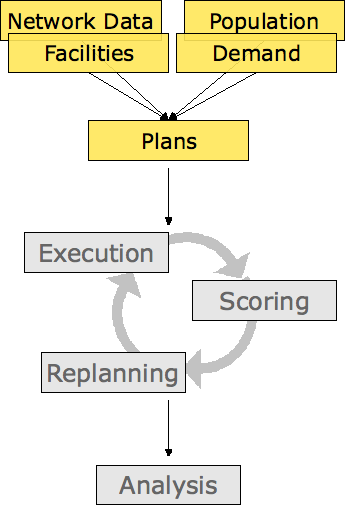
\includegraphics[width=4cm]{../graphics/overviewMatsimDemand.png}

\end{columns}

\end{frame}

\subsection{The Equil Scenario}


\begin{frame}[fragile]
\frametitle{Scenarios}
\framesubtitle{Equil Network}
\begin{itemize}
  \item Equil scenario:
  \begin{itemize}
  	\item \verb|./examples/equil/|
  \end{itemize}
  \item Start visualizer
  \begin{itemize}
  	\item Main method in \verb|org.matsim.utils.vis.netvis.NetVis|
  \end{itemize}
  \item Take a look at network
  \begin{itemize}
  	\item \verb|./examples/equil/network.xml|
  \end{itemize}
\end{itemize}
\end{frame}

\section{Running the examples}

\subsection{Running a single iteration}

\begin{frame}[fragile]
\frametitle{Running the examples}
\framesubtitle{Running a single iteration}
\begin{columns}[T]

\column{7cm}

\begin{itemize}
  \item 100 Agents from link 1 to 20
  \item Later from link 20 to 1
  \item Have a look at equil\_plans.xml
  \item Run \verb|org.matsim.run.Controler| with argument \verb|examples/tutorial/| \verb|singleIteration.xml|
  \item Examine the log for errors
\end{itemize}

\column{5cm}
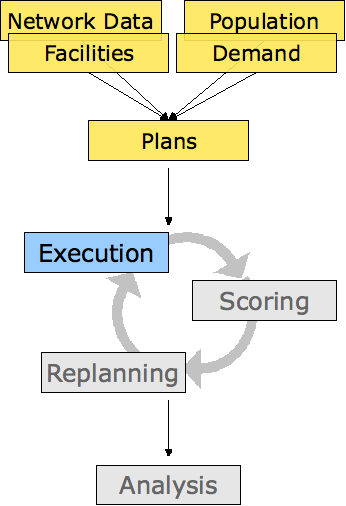
\includegraphics[width=4cm]{../graphics/overviewMatsimExecution.png}

\end{columns}

\end{frame}

\subsection{Visualizing the simulation results}

\begin{frame}[fragile]
\frametitle{Running the examples}
\framesubtitle{Visualizing the simulation results}
\begin{itemize}
  \item Start Netvis again
  \item Open file \verb|output/ITERS/it.0/SnapshotCONFIG.vis|
  \item Change daytime to 06:00 o'clock
  \item Increase linewidth
  \item Press play
  \item Read corresponding events at \verb|output/ITERS/it.0/0.events.txt|
\end{itemize}
\end{frame}


\subsection{Modifying the settings}

\begin{frame}[fragile]
\frametitle{Running the examples}
\framesubtitle{Modifying the settings}

\begin{itemize}
  \item Open \verb|examples/tutorial/singleIteration.xml|
  \item Try to change settings in the module simulation, e.g. endTime of 07:00 or snapshotperiod
  \item Run the simulation again
  \item Be aware of the error: \verb|The simulation will not overwrite files|
  \item Make snapshots in ``googleearth'' mode
\end{itemize}
\end{frame}


\subsection{Running multiple iterations}

\begin{frame}[fragile]
\frametitle{Running the examples}
\framesubtitle{Running multiple iterations}

\begin{columns}[T]

\column{7cm}

\begin{itemize}
  \item Use configuration \verb|examples/tutorial/multipleIterations.xml|
  \item Run controler
  \item 10 Iterations run with 10 \%  agents replanning
  \item Take a look at results
  \item Compare configuration files
  \item Increase number of iterations
\end{itemize}

\column{5cm}
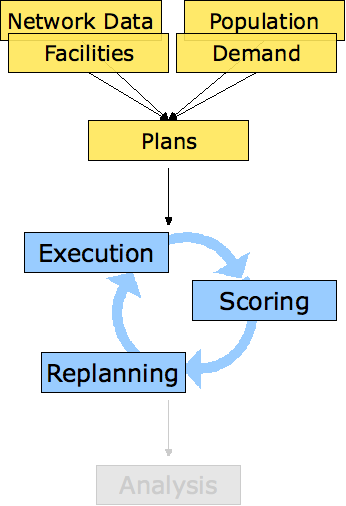
\includegraphics[width=4cm]{../graphics/overviewMatsimIterations.png}

\end{columns}

\end{frame}

\subsection{Modifying the re--planning}

\begin{frame}[fragile]
\frametitle{Running the examples}
\framesubtitle{Modifying the re--planning}

\begin{columns}[T]

\column{7cm}

\begin{itemize}
  \item Change \verb|ModuleProbability_2| in \verb|multipleIterations.xml| to 0.9
  \item Change \verb|ModuleProbability_1| to 0.1
  \item Run simulation again and look at results
  \item Replace value of \verb|Module_2| with \verb|TimeAllocationMutator|
  \item Examine results
  \item Combine the 3 re--routing strategies
\end{itemize}

\column{5cm}
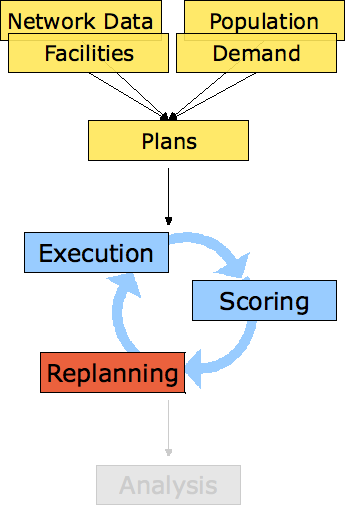
\includegraphics[width=4cm]{../graphics/overviewMatsimReplanning.png}

\end{columns}

\end{frame}


\section{Creating a custom controler}

%sub\subsection{Introduction}
\begin{frame}
\frametitle{Creating a custom controler}
\framesubtitle{Introduction}
\begin{itemize}
  \item Custom controler for
    \begin{itemize}
  	  \item Integration of own code
  	  \item Customized analysis
  	  \item More complex scenarios which require special modules
    \end{itemize}
  \item Only rewrite the parts you need, but try!
\end{itemize}
\end{frame}

%sub\subsection{First, helpful steps}

\begin{frame}[fragile]
\frametitle{Creating a custom controler}
\framesubtitle{First, helpful steps}
\begin{itemize}
  \item Inherit from \verb|Controler| and add main(String[] args)
  \item Create an instance and call \verb|setOverwriteFiles(true)|
  \item Call the \verb|Controler.run()| method
  \item Open visualizer after \verb|run()| is terminated
  \begin{verbatim}
String[] visargs = {"../output/ITERS/it.0/Snapshot"};
NetVis.main(visargs);\end{verbatim}
\end{itemize}

\end{frame}

%sub\subsection{Handling simulation events}

\begin{frame}[fragile]
\frametitle{Creating a custom controler}
\framesubtitle{Handling simulation events}
\begin{itemize}
  \item Simulation events output of simulation (physical world)
  \item Controler attribute \verb|protected final Events events|
  \item Handler interfaces in \verb|org.matsim.events.handler|
\end{itemize}

\end{frame}

\begin{frame}[fragile]
\frametitle{Creating a custom controler}
\framesubtitle{Handling simulation events}
\begin{itemize}
  \item Write own handler \\
  \begin{verbatim}
MyHandler implements EventhandlerLinkLeave {
  public void handleEvent (EventLinkLeave event) {
    	...do something...
  }
  public void reset(int iteration) {
    	...reset something...
  }
}\end{verbatim}
\end{itemize}

\end{frame}

%sub\subsection{Handling simulation events}

\begin{frame}[fragile]
\frametitle{Creating a custom controler}
\framesubtitle{Handling simulation events}
\begin{itemize}
  \item Create an instance \\
  \begin{verbatim}
  MyHandler handler = new MyHandler();
  \end{verbatim}
  \item Register at Events instance \\
  \begin{verbatim}
  events.addHandler(handler);
  \end{verbatim}
 \end{itemize}
\end{frame}

%sub\subsection{Handling controler events}

\begin{frame}
\frametitle{Creating a custom controler}
\framesubtitle{Handling controler events}
\begin{itemize}
  \item Controler events output of simulation process, e.g.
  \begin{itemize}
  	\item Startup complete
  	\item Begin iteration
  	\item End iteration
  	\item Replanning
  	\item Shutdown
  \end{itemize}
\end{itemize}
\end{frame}


\begin{frame}[fragile]
\frametitle{Creating a custom controler}
\framesubtitle{Handling controler events}
\begin{itemize}
  \item Interfaces in \verb|org.matsim.controler.listener|
  \item Implement and add by \\
  \begin{verbatim}
Controler.addControlerListener(myListenerInstance);
  \end{verbatim}
\end{itemize}

\end{frame}

\begin{frame}[fragile]
\frametitle{Creating a custom controler}
\framesubtitle{Analyse results}
\begin{columns}[T]

\column{7cm}

\begin{itemize}
  \item Controler generates some analysis
  \begin{itemize}
    \item Score statistics
    \item Plans (per 10th iteration)
    \item Snapshots (per 10th iteration)
  	\item Leg histograms (per iteration)
  \end{itemize}
  \item Customized charts via Event handler / listener
  \item Useful tool: \verb|org.matsim.utils.charts|
\end{itemize}

\column{5cm}
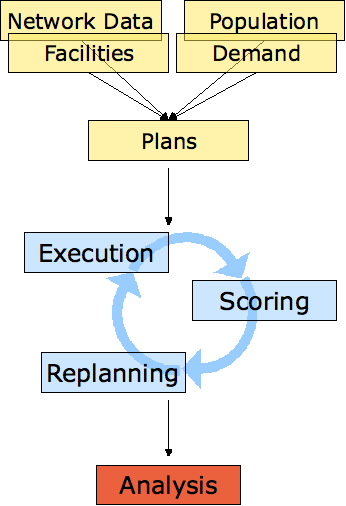
\includegraphics[width=4cm]{../graphics/overviewMatsimAnalysis.png}

\end{columns}
\end{frame}


\section{Outlook}

\subsection{Next steps for Advest}

\begin{frame}
\frametitle{Outlook}
\framesubtitle{Next steps for Advest}
\begin{itemize}
  \item VSP will provide 1\%, 10\%, 100\% input data for
  \begin{itemize}
  	\item Traffic light control
  	\item Evacuation scenarios
  \end{itemize}
  \item VSP runs big scenarios
  \item Further questions and tasks?
\end{itemize}
\end{frame}

\end{document}
